\documentclass[12pt]{article}
\usepackage{amsmath,amsfonts,times}
\usepackage{graphicx,color,tikz,pgfplots}
\usepackage[paperwidth=8.1cm,paperheight=8.1cm,lmargin=0in,rmargin=0in,tmargin=0.in,bmargin=0.in]{geometry}
\usepackage{bm}
\usetikzlibrary{arrows,shadings,shapes.arrows,decorations.pathreplacing,calc, positioning}
\usepgfplotslibrary{fillbetween}

\begin{document}
\centering

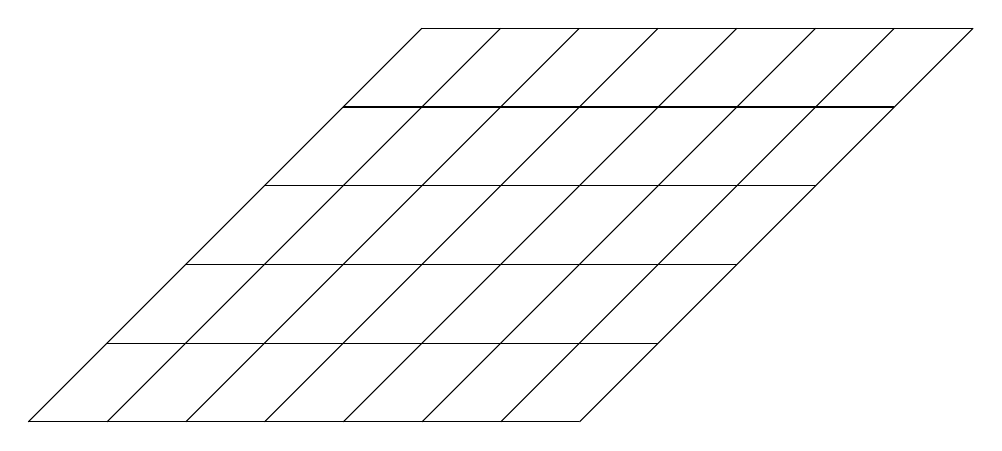
\begin{tikzpicture}[on grid]
  \newcommand{\slantedgrid}[4]{%
    \pgfmathtruncatemacro{\result}{#1+#3}
    \foreach \x in {#1,...,\result} \draw (\x,#2) -- ++(#4,#4);%
    \pgfmathtruncatemacro{\result}{#2+#4}
    \foreach \y in {#2,...,\result} \draw (#1+\y-#2,\y) -- ++(#3,0);%
  }
  \slantedgrid{10}{12}{7}{5}
\end{tikzpicture}

\end{document} 
